\chapter{Uso del prototipo}
En este cap\'itulo hacemos uso del prototipo desarrollado para el poblado de datos de prueba para una base de datos, para lo cual es necesario que se tenga cantidad de tablas.
Como ejemplo tomamos  una base de datos denominada prueba como observamos en la Figura \ref{fig:createDatabase}

\begin{figure}[H]
\caption{Base de datos prueba} \label{fig:createDatabase}
\centering
\subfigure{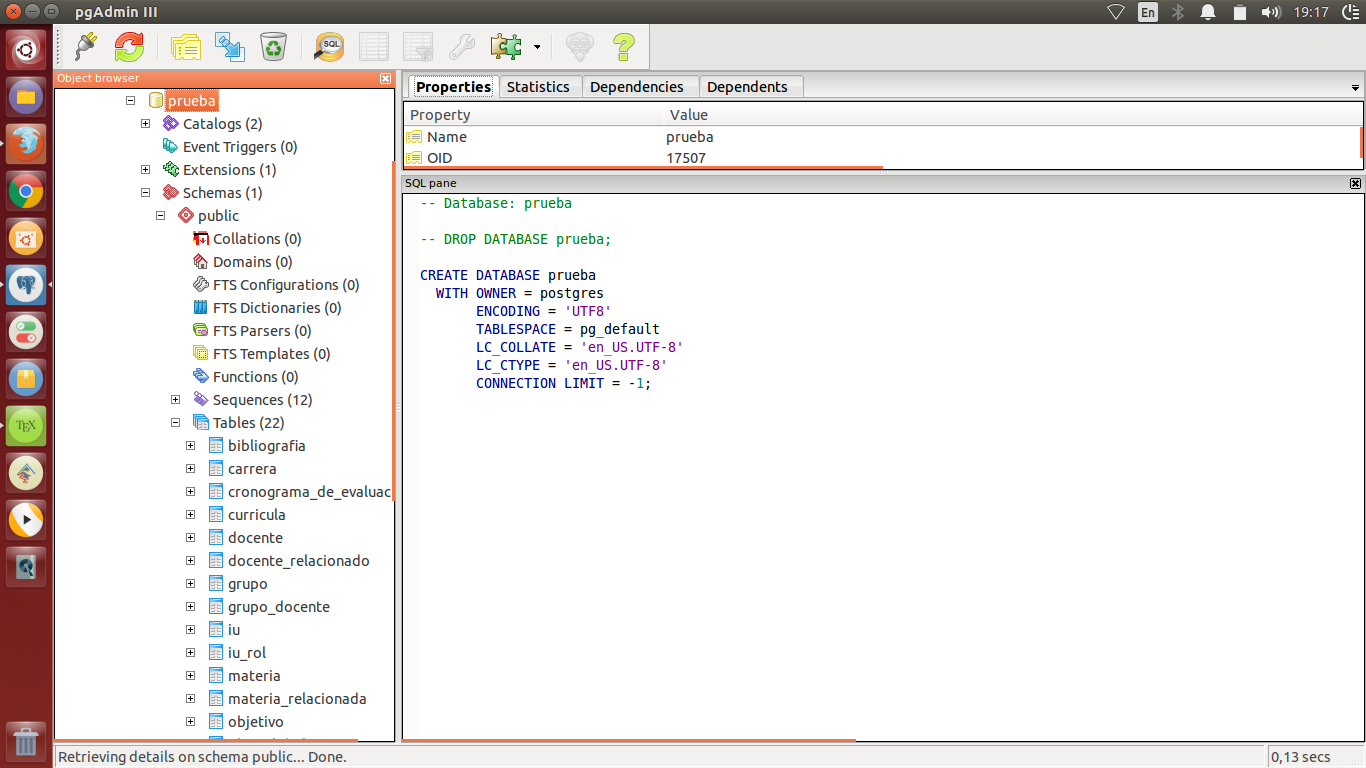
\includegraphics[scale=0.3]{images/prototipo/0-createDatabase.png}}
\end{figure}

Esta base de datos se tiene veinte y dos tablas como se observa en la Figura \ref{fig:listatablePrueba}. 
\begin{figure}[H]
\caption{Base de datos prueba} \label{fig:listatablePrueba}
\centering
\subfigure{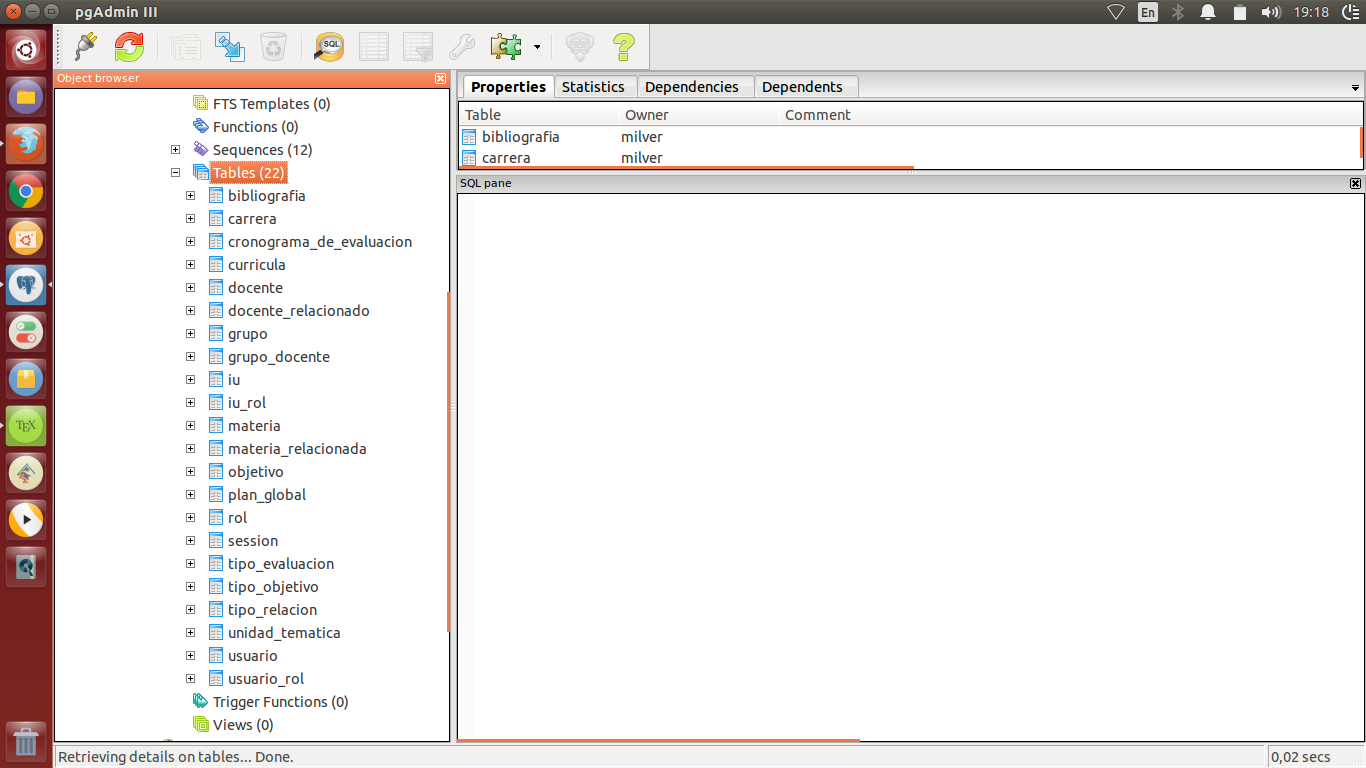
\includegraphics[scale=0.3]{images/prototipo/1-listTables.png}}
\end{figure}

En el prototipo se tiene la opci\'on de crear como un proyecto en el boton nuevo y la lista de proyectos como se ve en la Figura \ref{fig:homePototype}.
\begin{figure}[H]
\caption{Lista de proyectos} \label{fig:homePototype}
\centering
\subfigure{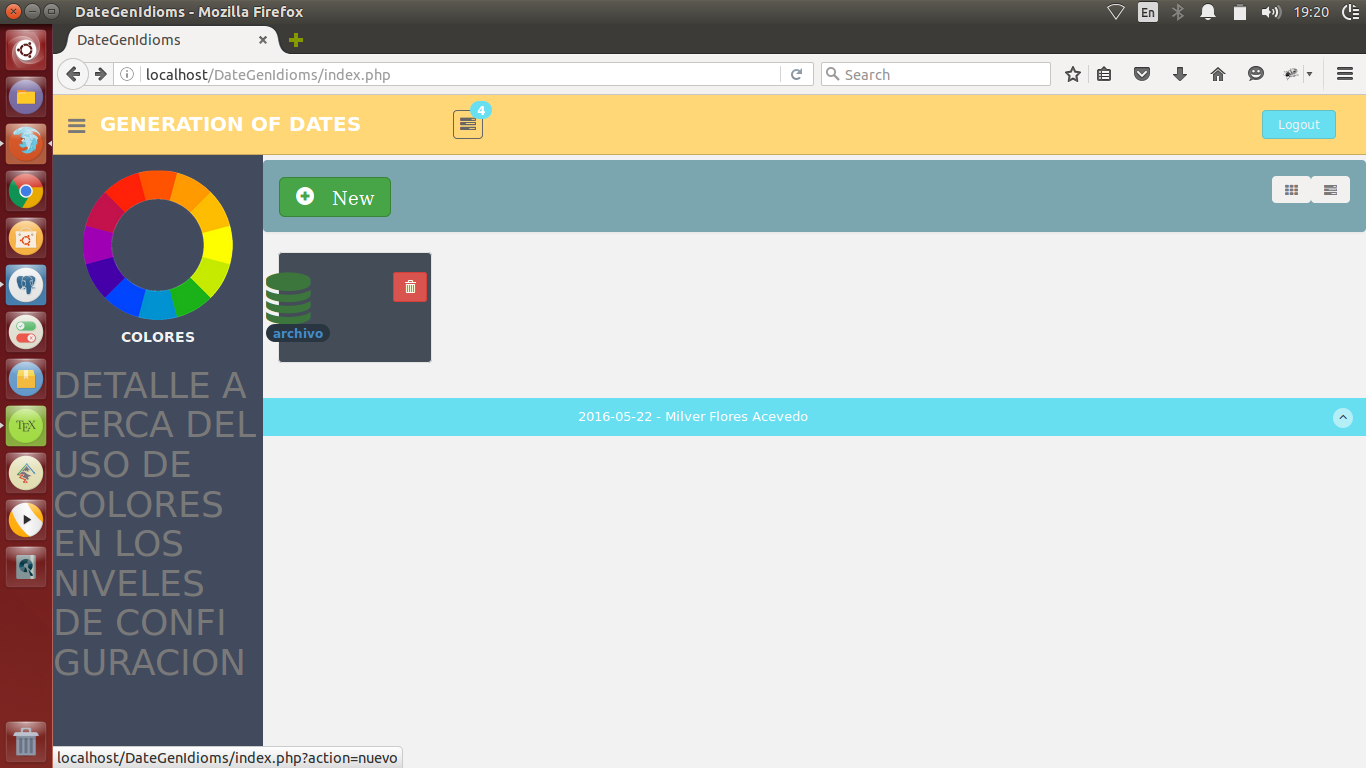
\includegraphics[scale=0.3]{images/prototipo/2-createNewProject.png}}
\end{figure}

Al hacer clic nos llevara a un formulario como se ve en la Figura \ref{fig:formnewproject}
\begin{figure}[H]
\caption{Formulario para crear un nuevo proyecto} \label{fig:formnewproject}
\centering
\subfigure{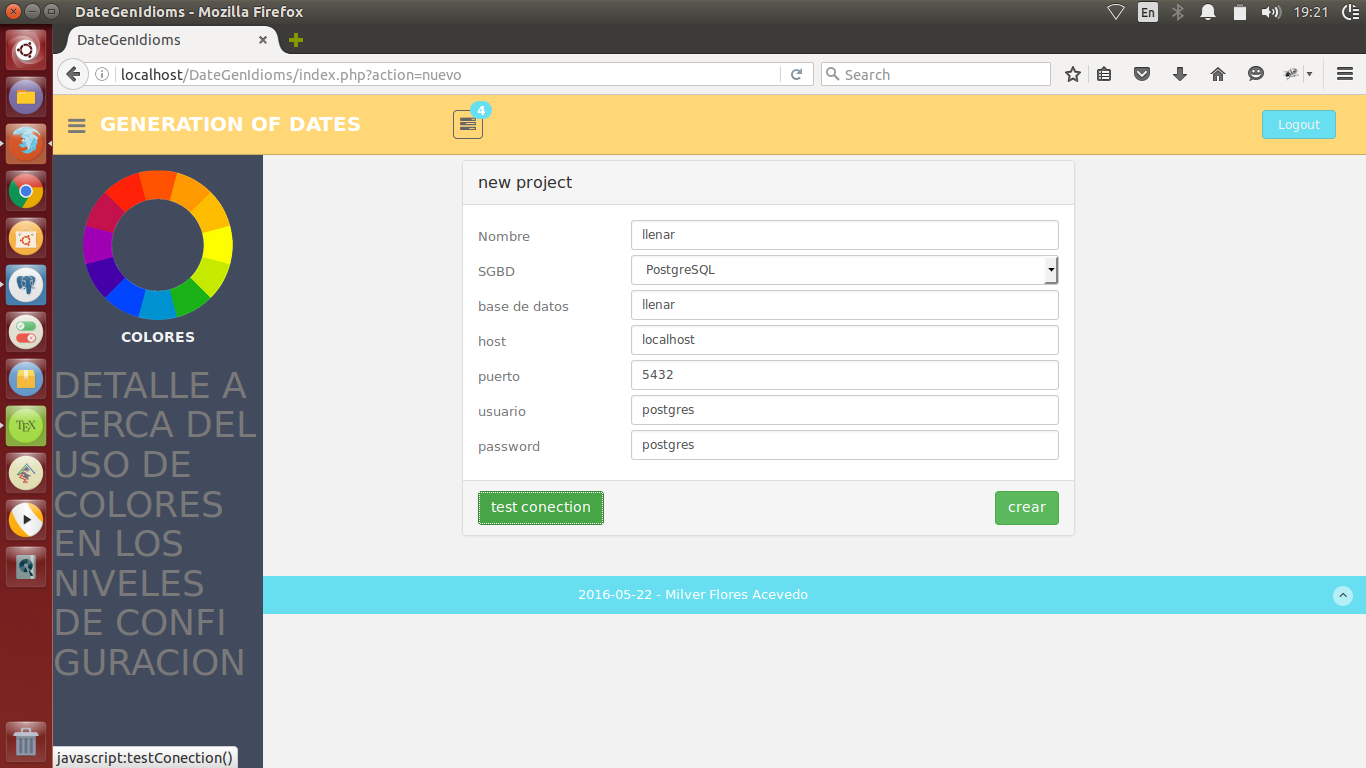
\includegraphics[scale=0.3]{images/prototipo/3-fillFieldsToConnect.png}}
\end{figure}
Para crear un proyecto es necesario llenar los datos en el formulario que son:

\begin{description}[align=left]
\item [Nombre] este campo es a eleccion con la restricci\'on que no se puede tener dos proyectos con el mismo nombre.
\item [sgbd] el sistema gestor de base de datos que en este trabajo elegimos trabajar con PostgreSQL.
\item [base de datos] en este campo es necesario el nombre exacto de la base de datos por que sera de la cual obtendremos su estructura.
\item [host] la url donde se encuentra alojada la base de datos. En nuestro caso localhost.
\item [puerto] normalmente el puerto que usa PostgreSQL es 5432.
\item [usuario] con el usuario que se conectara con previligios de acceso a metadatos.
\item [password] la contrase\~na del usuario
\end{description}
\begin{figure}[H]

\caption{Conexion exitosa} \label{fig:connectionsuccessfull}
\centering
\subfigure{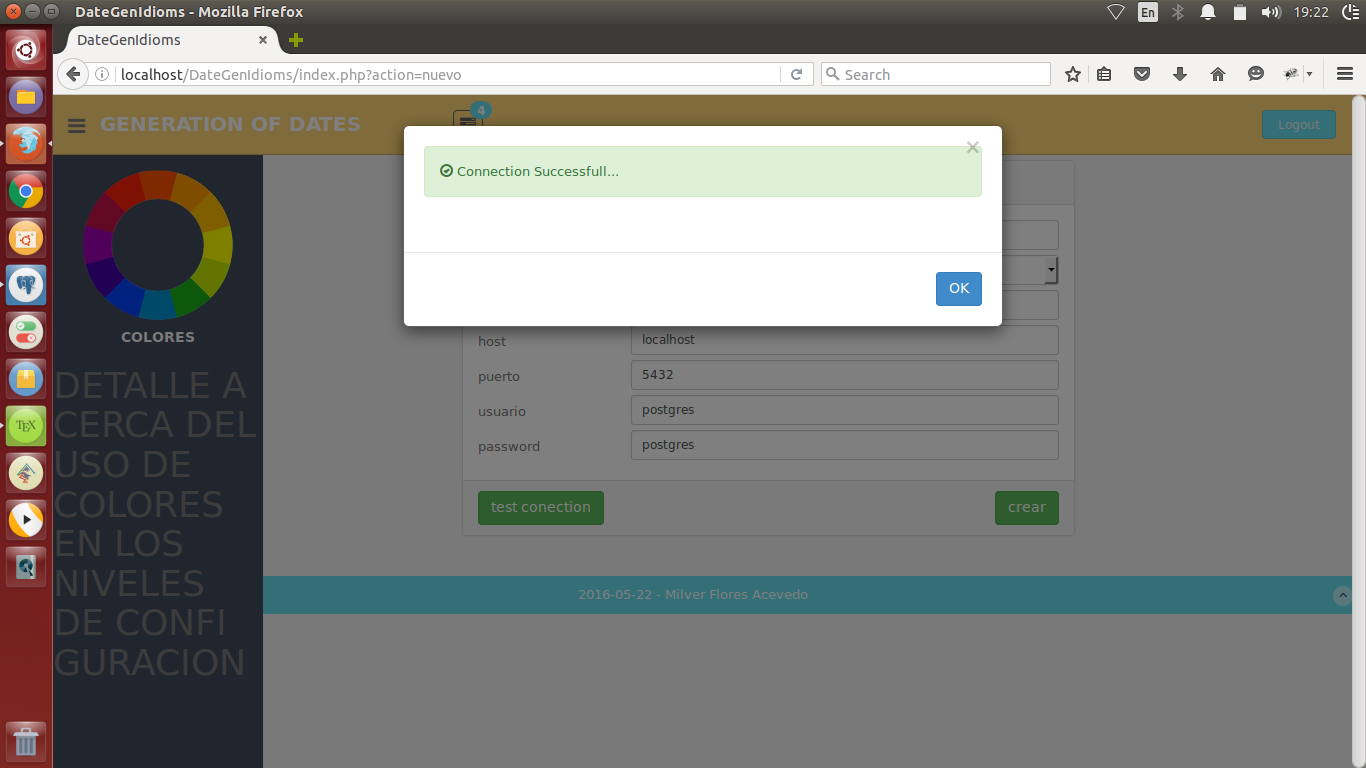
\includegraphics[scale=0.3]{images/prototipo/4-testConnection.png}}
\end{figure}
Una vez llenada el formulario lo siguente es probar la conexion dando clic en el boton de test connection, si es exitosa muestra el mensaje de una conexion exitosa. 
\begin{figure}[H]
\caption{Boton crear} \label{fig:createbutton}
\centering
\subfigure{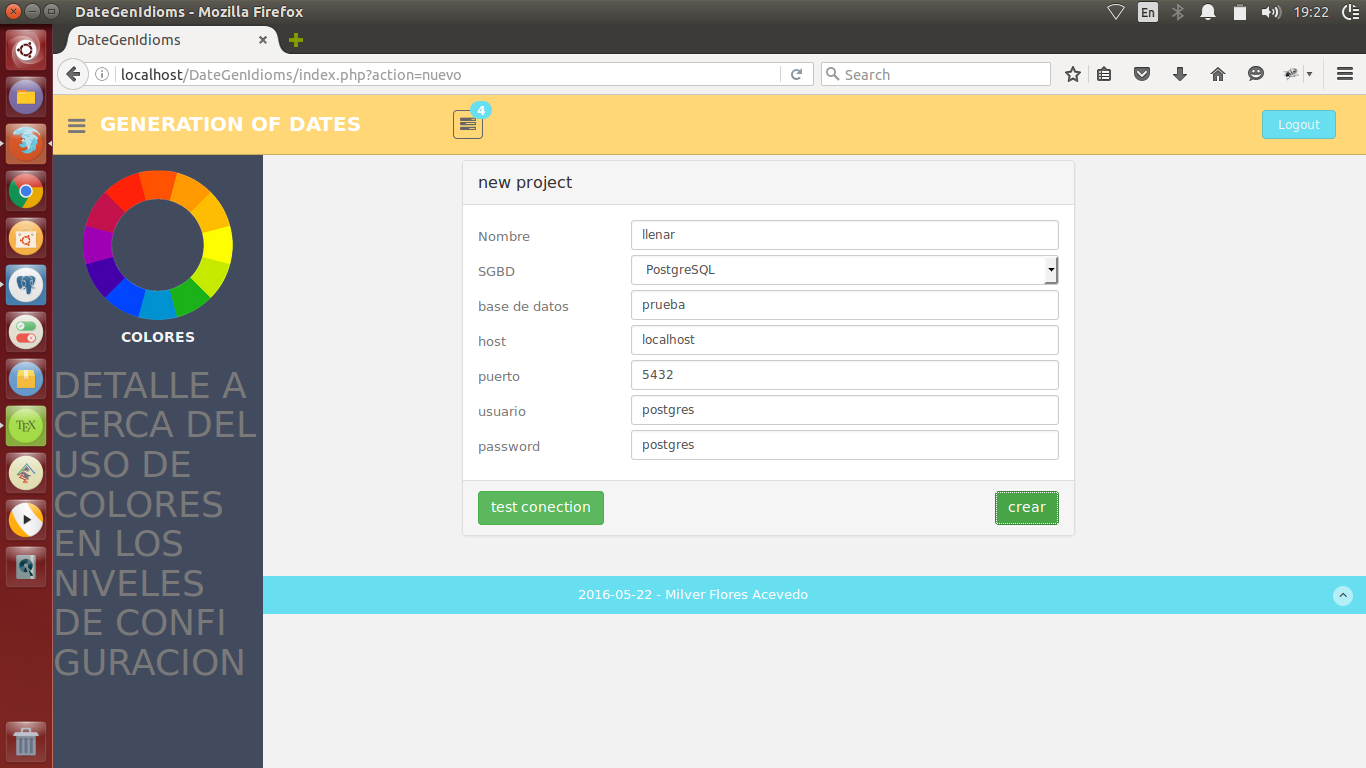
\includegraphics[scale=0.3]{images/prototipo/5-OkCreateProject.png}}
\end{figure}
Si los datos del formulario son correctas damos clic en el boton crear ver Figura \ref{fig:createbutton}, a continuaci\'oin nos redirigir\'a a la lista de proyectos en la cual aparecera el proyeto que creamos. 
\begin{figure}[H]
\caption{Proyecto creado} \label{fig:viewprojectcreated}
\centering
\subfigure{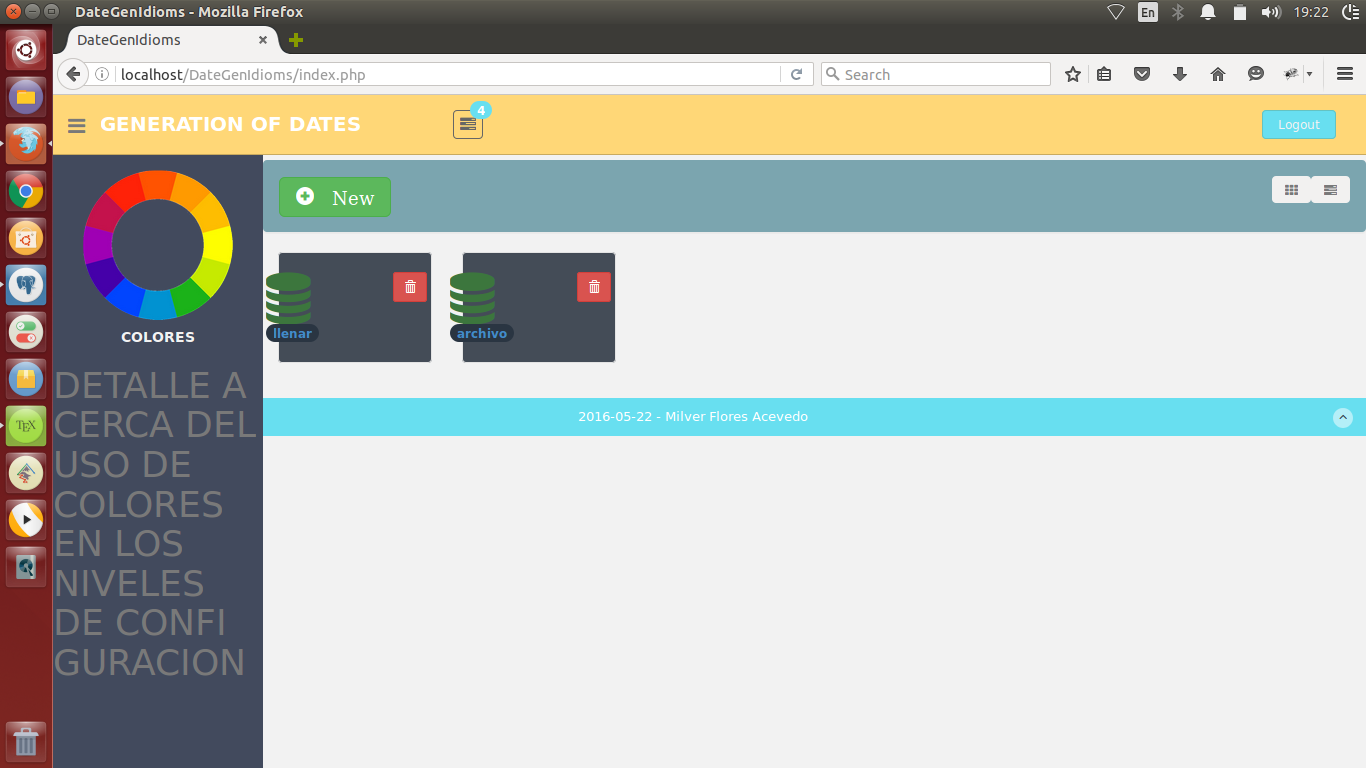
\includegraphics[scale=0.3]{images/prototipo/6-viewProjectCreated.png}}
\end{figure}
A continuacion damos clic en el nombre del proyeto lo cual no muestra toda la estructura del proyecto creado y ahi tenemos listo con el orden en que se debe llenar la base de datos iniciando primero todos los que son de color verde terminando con los rojos.
\begin{figure}[H]
\caption{7}
\centering
\subfigure{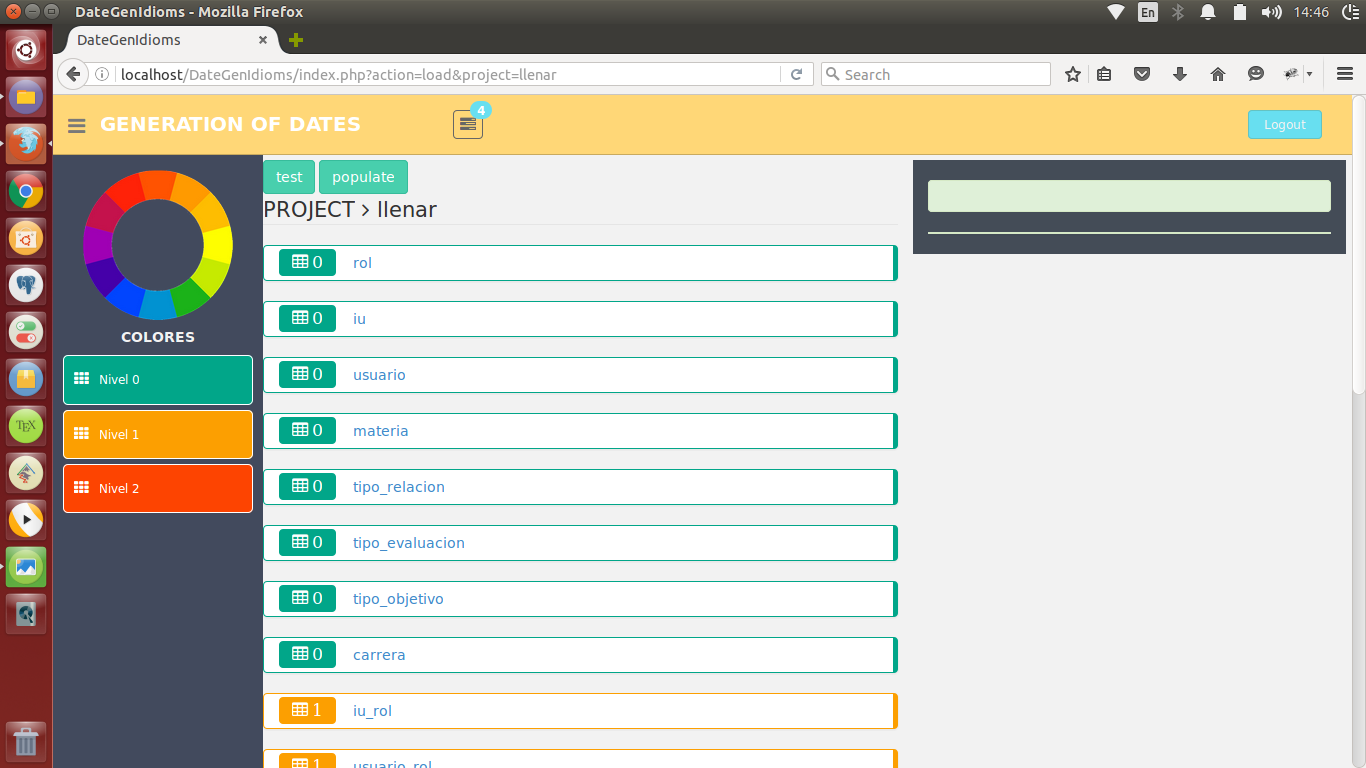
\includegraphics[scale=0.3]{images/prototipo/7-viewListTablesUI.png}}
\end{figure}
Si observamos en la Figura \ref{fig:detalletablerol} se tiene \texttt{id\_rol, nombre}, donde \texttt{id\_rol} es la llave primaria por lo cual este tipo de datos se genera en un cierto rango de n\'umero.

\begin{figure}[H]
\caption{9}
\centering
\subfigure{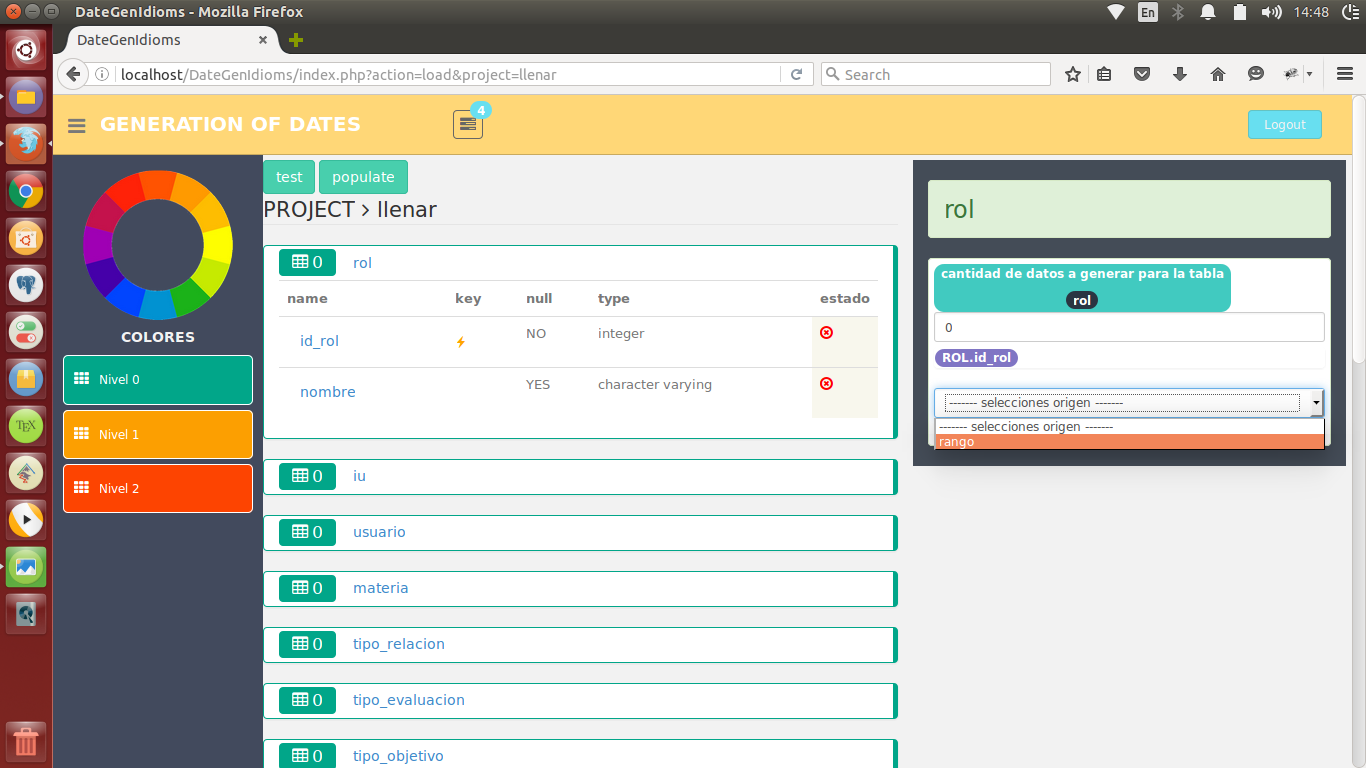
\includegraphics[scale=0.3]{images/prototipo/9-viewTypeFieldAndListOptionFill.png}}
\end{figure}
Seg\'un el tipo de dato el formulario tiene una variaci\'on y las opciones que ofrece como queremos generarlo,
para el caso de \texttt{id\_rol} al ser una llave primaria tenemos la opcion de generar en un cierto rango de numeros.
\begin{figure}[H]
\caption{10}
\centering
\subfigure{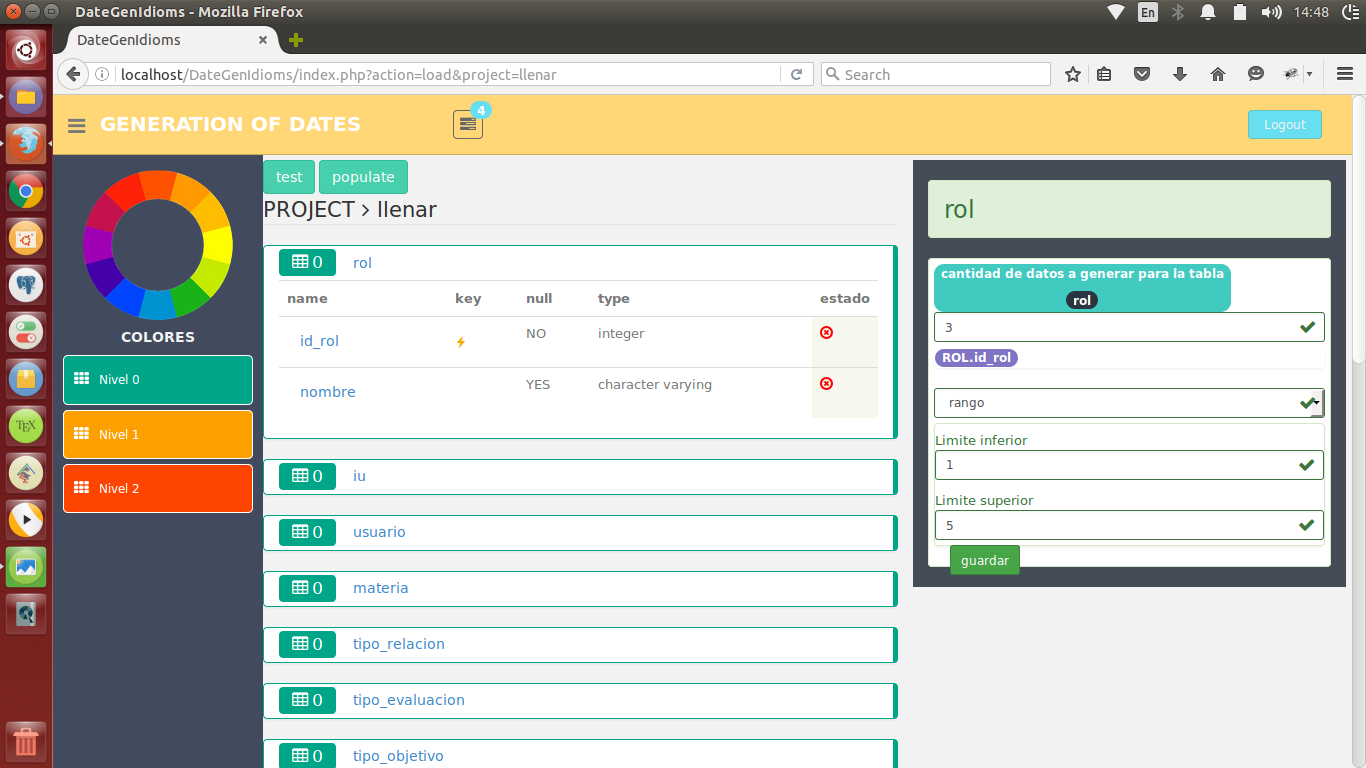
\includegraphics[scale=0.3]{images/prototipo/10-fillFieldsForTable.png}}
\end{figure}
Una vez llenada el formulario damos clic en guradar.
\begin{figure}[H]
\caption{11}
\centering
\subfigure{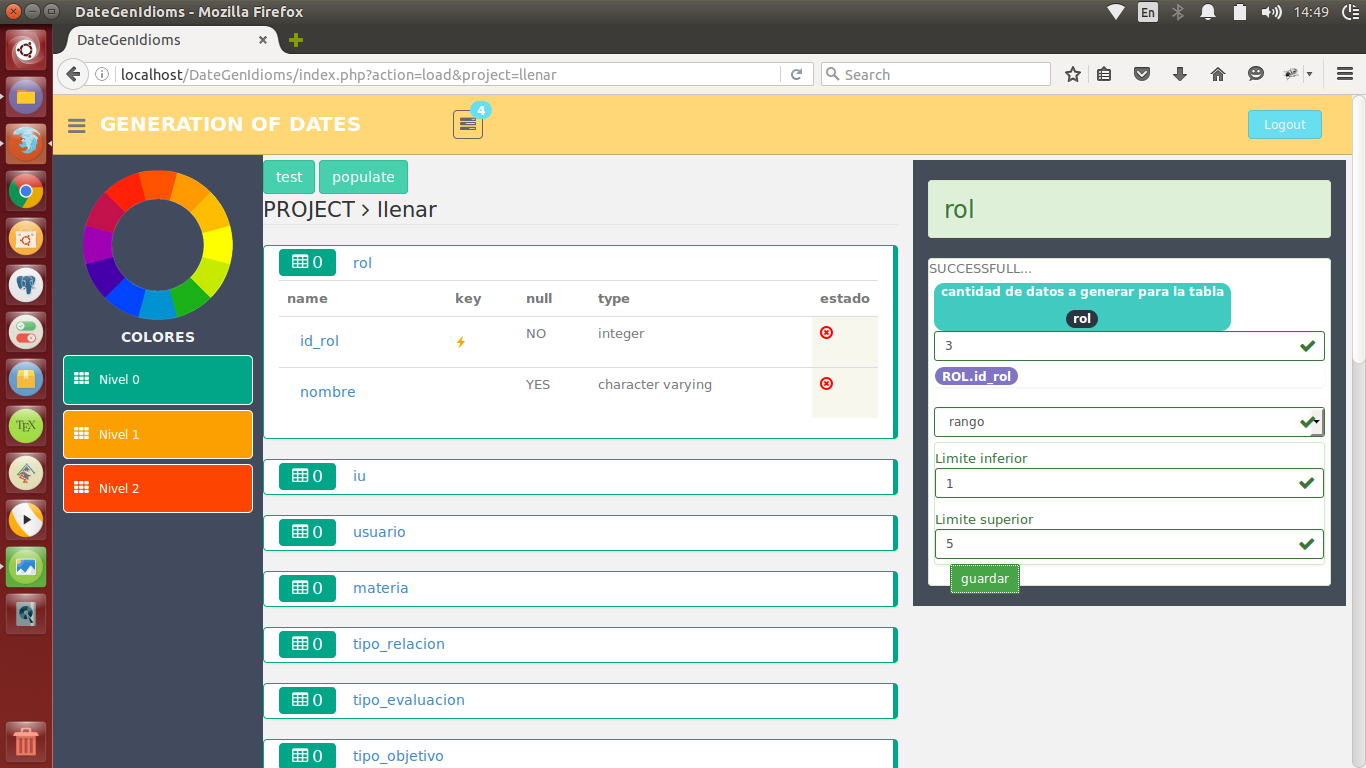
\includegraphics[scale=0.3]{images/prototipo/11-OKFillAndMessageSuccess.png}}
\end{figure}
Ahora veamos a una tabla que haga referencia \texttt{usuario\_rol} donde no es necesario llenar formularios.
\begin{figure}[H]
\caption{12}
\centering
\subfigure{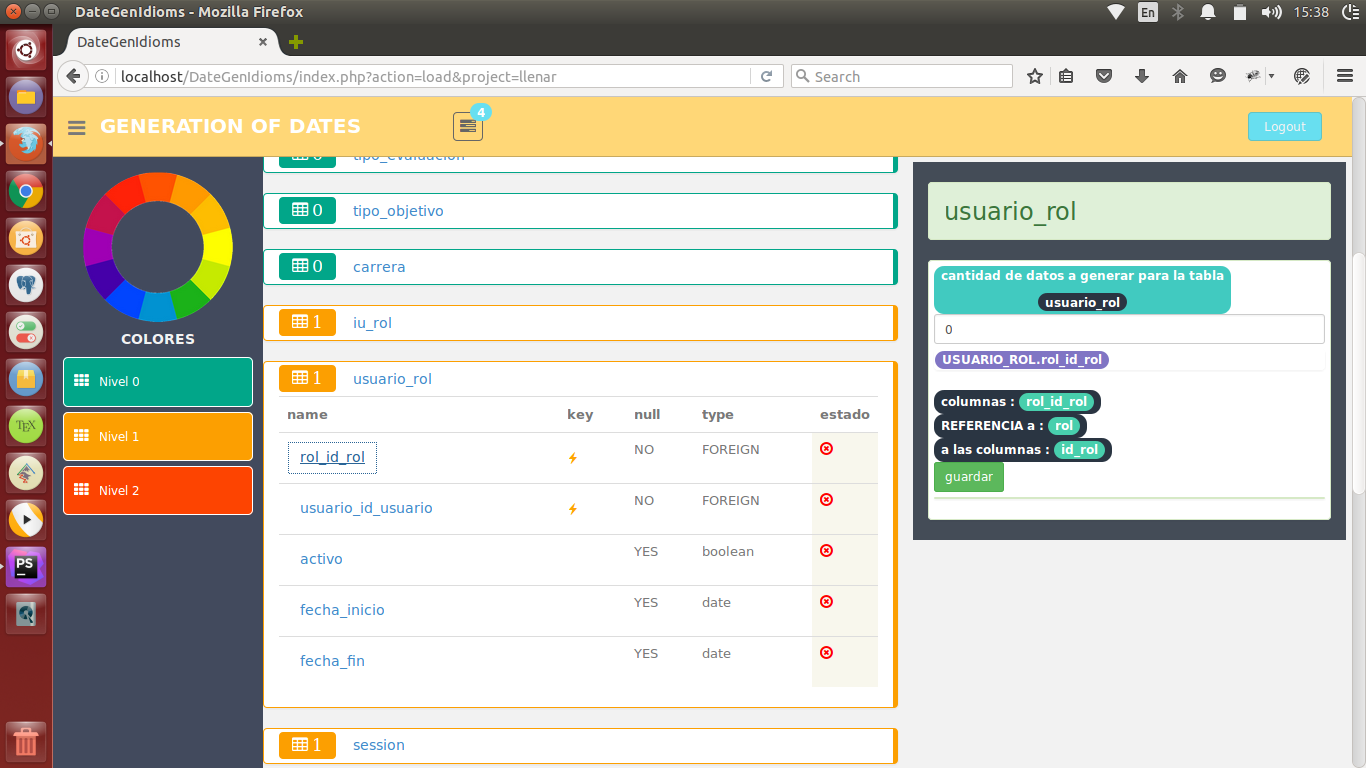
\includegraphics[scale=0.3]{images/prototipo/17-usuario-rol.png}}
\end{figure}
Una vez que se conpleta la configuraci\'on de todas las tablas damos clic en el boton test y como podemos observar en la Figura \ref{fig:statusConnection}
\begin{figure}[H]
\caption{Estado de configuracion}\label{fig:statusConnection}
\centering
\subfigure{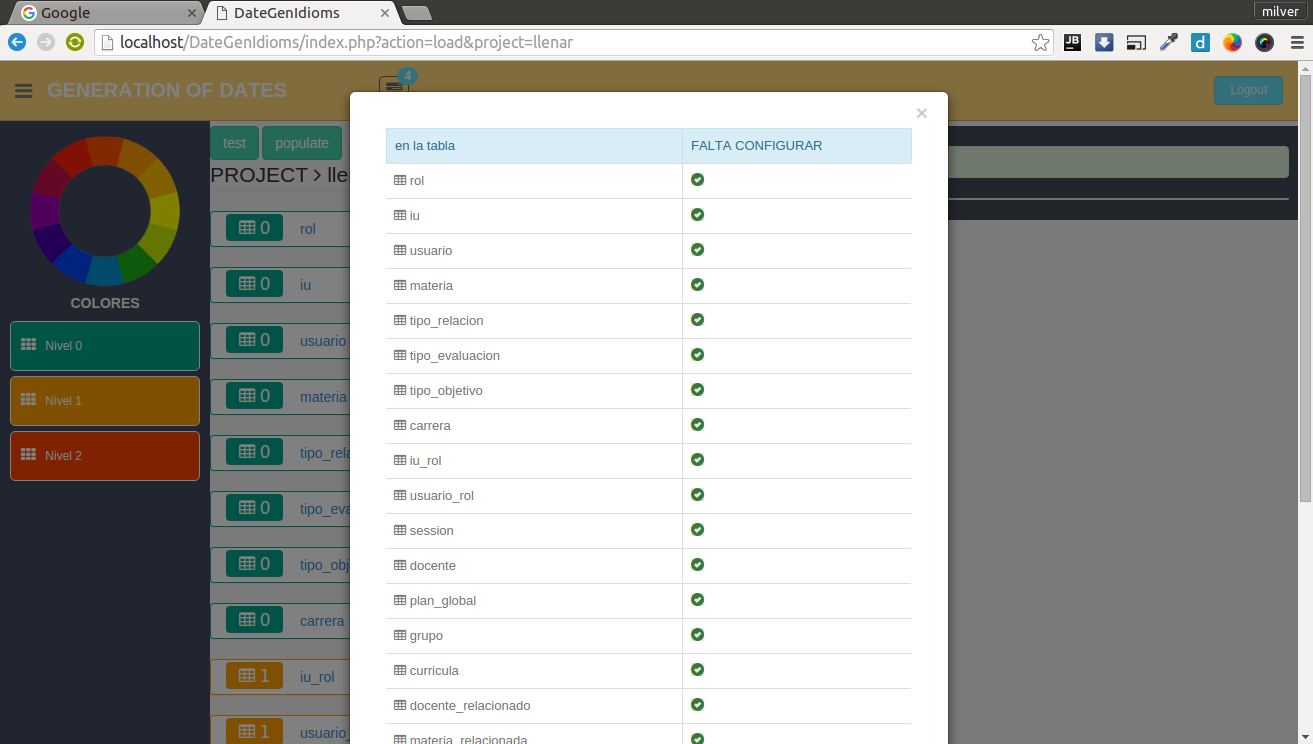
\includegraphics[scale=0.3]{images/prototipo/viewStatusSettings.png}}
\end{figure}
 Si se tiene toda la configuraci\'on ya se puede llenar la base de datos dando clic en el boton populate, esperamos que haga el llenado para posteriormente ver como se ven reflajado en la base de datos.
 
 \begin{figure}[H]
\caption{Llenando la base de datos}\label{fig:populating}
\centering
\subfigure{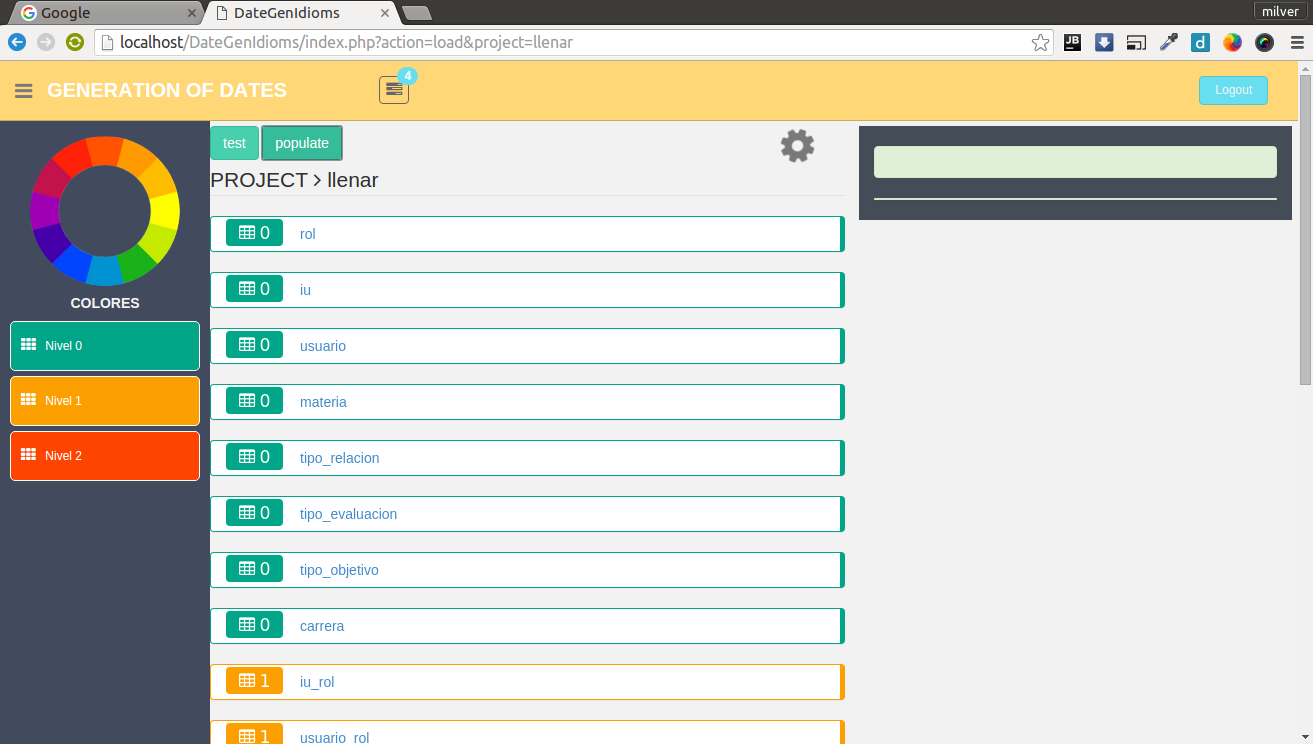
\includegraphics[scale=0.3]{images/prototipo/populating.png}}
\end{figure}
Si vemos en la base de datos la tabla \texttt{docente} ya se tiene datos de prueba como vemos en la Figura \ref{fig:tableDocente}
\begin{figure}[H]
\caption{Tabla docente}\label{fig:tableDocente}
\centering
\subfigure{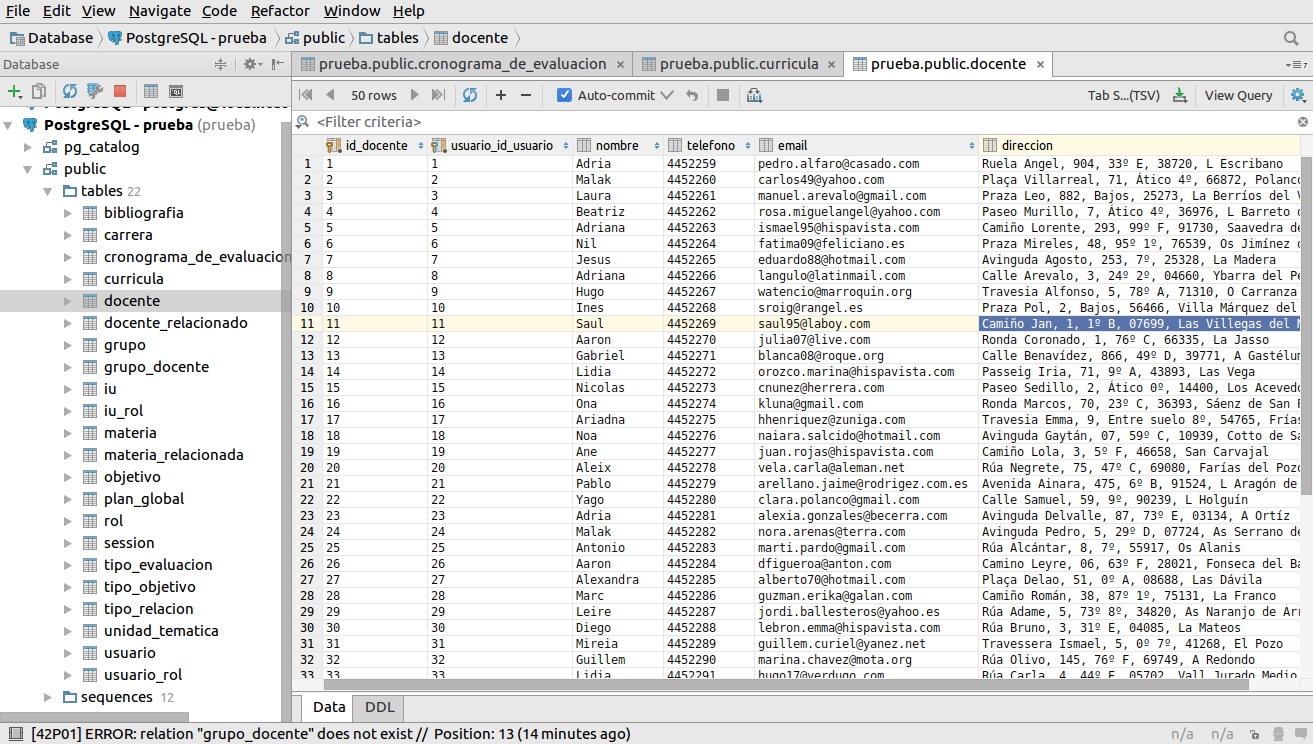
\includegraphics[scale=0.3]{images/prototipo/filledTableDocente.png}}
\end{figure}
pasa lo mismo con la tabla \texttt{rol} podemos observar los tres datos que ingresamos.
\begin{figure}[H]
\caption{Tabla rol}\label{fig:tableRol}
\centering
\subfigure{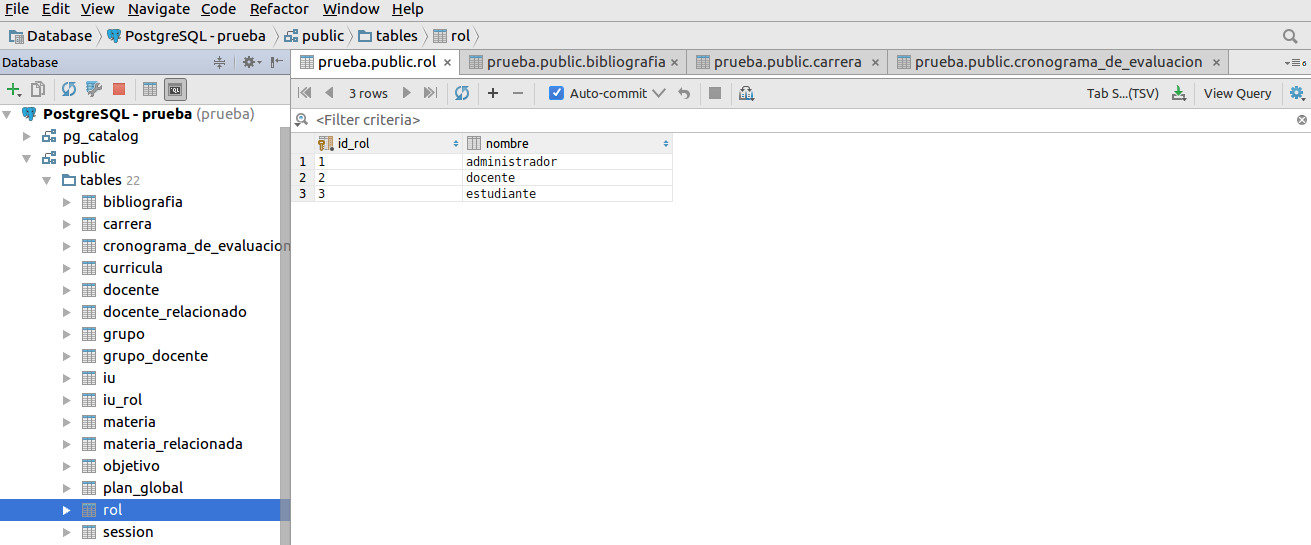
\includegraphics[scale=0.3]{images/prototipo/filledTableRol.png}}
\end{figure}
si se tiene la misma base de datos en distintas maquinas podemos usar el sql generado por el generador.
\begin{figure}[H]
\caption{Sql generado}\label{fig:sqlGenerated}
\centering
\subfigure{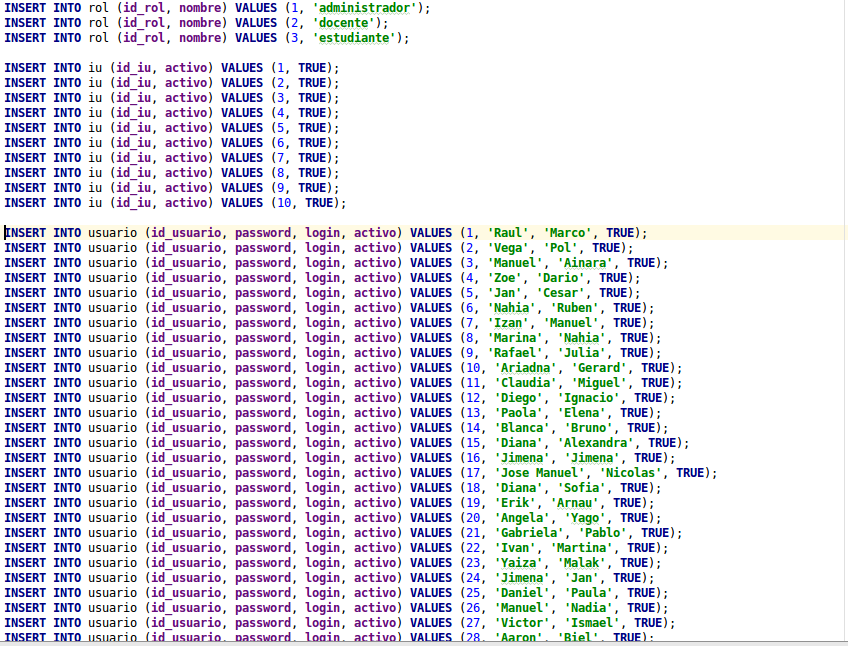
\includegraphics[scale=0.55]{images/prototipo/sql.png}}
\end{figure}





